\documentclass[12pt,number,sort&compress,preprint]{elsarticle}

%======================================================================
\usepackage{todonotes}
\usepackage{graphicx}
\usepackage[binary-units]{siunitx}
\usepackage{gensymb}
\usepackage[version=3]{mhchem} % Formula subscripts using \ce{}, e.g., \ce{H2SO4}
\usepackage{booktabs,multicol} %better tables
\usepackage{subcaption} %subfigs
\usepackage{lmodern}
\usepackage[T1]{fontenc}
\usepackage{textcomp}

% shared equations in separate file
% https://yatb.giacomodrago.com/en/post/3/latex-loading-equations-from-an-external-file.html
\usepackage{catchfilebetweentags}

\newcommand{\loadeq}[1]{%
   \ExecuteMetaData[eqn_dict.tex]{eq#1}%
}

% external references https://tex.stackexchange.com/a/14365/56227
\usepackage{xr-hyper}

\usepackage{amsmath,eqparbox,xparse}

\usepackage[breaklinks=true, linkcolor=blue, citecolor=blue, colorlinks=true]{hyperref}
% load after hyperref
\usepackage[english,capitalise]{cleveref}


%%%%%%%%%%%%%%%%%%%%%%%%%%%%
%      Custom Commands     %
%%%%%%%%%%%%%%%%%%%%%%%%%%%%


% https://tex.stackexchange.com/a/34412/5764
\makeatletter
\NewDocumentCommand{\eqmathbox}{o O{c} m}{%
  \IfValueTF{#1}
    {\def\eqmathbox@##1##2{\eqmakebox[#1][#2]{$##1##2$}}}
    {\def\eqmathbox@##1##2{\eqmakebox{$##1##2$}}}
  \mathpalette\eqmathbox@{#3}
}
\makeatother


\sisetup{group-separator={,},
	detect-all,
	binary-units,
	list-units = single,
	range-units = single,
	range-phrase = --,
	per-mode = symbol-or-fraction,
	separate-uncertainty = true,
	multi-part-units = single,
	list-final-separator = {, and }
	%    scientific-notation = fixed
}

% load external document after hyperref https://tex.stackexchange.com/a/281417/56227
\externaldocument[deriv-]{derivations}

%======================================================================
% Add your bibliography file here, replace template.bib
\bibliographystyle{elsarticle-num}

\newcommand{\pluseq}{\mathrel{{+}{=}}}
\newcommand{\minuseq}{\mathrel{{-}{=}}}
\newcommand{\ns}{N_{sp}}
\newcommand{\nr}{N_{reac}}
\newcommand{\conp}{CONP}
\newcommand{\conv}{CONV}
\newcommand{\dconp}{\ifmmode\text{for \conp,}\else for \conp,\fi}
\newcommand{\dconv}{\ifmmode\text{for \conv,}\else for \conv.\fi}
\newcommand{\Ru}{\mathcal{R}}

% simple command for equal-sized eqmathbox's on the lhs / rhs and conditional
% arguements are tag, text, alignment
\NewDocumentCommand{\lhs}{mmO{r}}{\eqmathbox[LHS_#1][#3]{#2}}
\NewDocumentCommand{\rhs}{mmO{l}}{\eqmathbox[RHS_#1][#3]{#2}}
\NewDocumentCommand{\cond}{mmO{r}}{\eqmakebox[COND_#1][#3]{#2}}
\NewDocumentCommand{\mathcond}{mmO{r}}{\eqmathbox[COND_#1][#3]{#2}}

% consistent multiline equation spacing
\NewDocumentCommand{\mathindent}{O{space}}{\hphantom{\mathrel{#1}}}

% set figure path
\graphicspath{{./figures/}}


\title{SIMD\slash SIMT-vectorized Sparse Chemical Kinetic Jacobian\slash Thermo-chemical Source Term Evaluation}

\author[1]{Nicholas Curtis\corref{corr}}
\ead{nicholas.curtis@uconn.edu}
\author[1]{Chih-Jen Sung}

\address[1]{Department of Mechanical Engineering, University of Connecticut, Storrs, CT 06269, USA}
\cortext[corr]{Corresponding author}

\begin{document}

\begin{frontmatter}

%====================================================================
\begin{abstract} % not to exceed 200 words
A code generation platform for single-instruction, multiple-data (SIMD) and single-instruction, multiple thread (SIMT) vectorized thermo-chemical source term and sparse chemical kinetic Jacobian evaluation was developed and validated for a wide range of chemical kinetic models.
\todo[inline]{this}
\end{abstract}

% (Provide 2-4 keywords describing your research. Only abbreviations firmly
% established in the field may be used. These keywords will be used for
% sessioning/indexing purposes.)
\begin{keyword}
    Chemical Kinetics\sep SIMD\sep SIMT\sep Vector Processing\sep Jacobian
\end{keyword}

\end{frontmatter}

%====================================================================
\section{Introduction}
%

Single-Instruction, Multiple-Data (SIMD) and the related Single-Instruction, Multiple-Thread (SIMT) processing are two important vector-processing paradigms used increasingly in scientific computing.
Traditional multi-core parallelism is often used to increase central processing unit (CPU) performance, however SIMD processors---as well as SIMT processors, e.g., in the form of graphics processing units (GPUs)---have gained recognition due to their increased floating operation throughput.
The parallel programming standard OpenCL~\cite{stone2010opencl} has further enabled adoption of vector-processing based codes in scientific computing by providing a common application program interface (API) for execution on heterogeneous systems, e.g., the CPU, GPU, or Intel's Many Integrated Core architecture (MIC), etc.
In this discussion, we will largely use OpenCL terminology to describe these processing paradigms, as it provides a convenient way to classify otherwise disparate processor type (e.g., CPUs and GPUs), however the concepts discussed are broadly applicable to SIMD\slash SIMT processing and not tied to OpenCL specifically.

\begin{figure}[htb]
  \centering
  \begin{subfigure}[htp]{0.45\linewidth}
      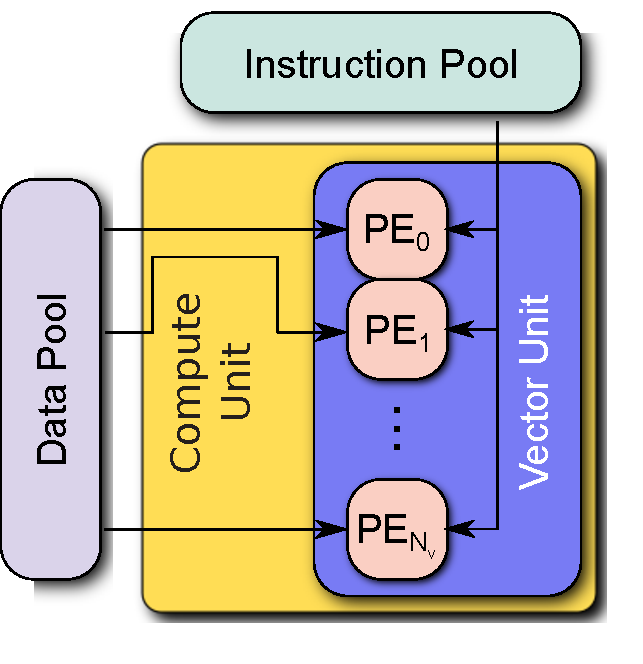
\includegraphics[width=\textwidth]{SIMD.pdf}
      \caption{Schematic of SIMD processing.  A single compute unit (e.g., a CPU core) contains a vector unit with $N_v$ processing elements, together called a vector-lane.  The vector unit executes a single instruction concurrently on multiple data.}
      \label{F:SIMD}
  \end{subfigure}
  \hfill
  \begin{subfigure}[htp]{0.45\linewidth}
      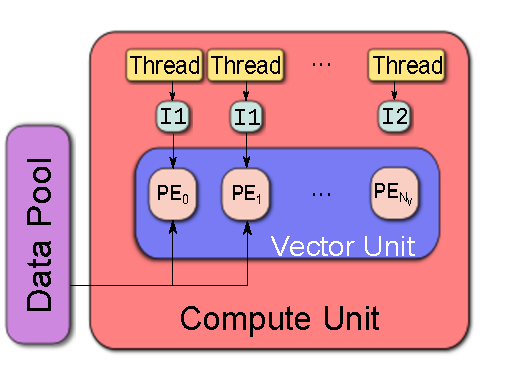
\includegraphics[width=\textwidth]{SIMT.pdf}
      \caption{Schematic of SIMT processing. A single compute unit (e.g., a GPU streaming multiprocessor) contains many processing elements and hosts many threads, each with an instruction to execute (I1, I2).  Threads with the same instruction execute concurrently on multiple data while the others must wait (leading to thread divergence).}
      \label{F:SIMT}
  \end{subfigure}
\end{figure}

A typical modern CPU has many compute units (i.e., cores), each with specialized vector processing units capable of running SIMD instructions (\cref{F:SIMD}).
A SIMD instruction utilizes the vector processor to execute the same floating point operation (e.g. multiplication, division, etc.) on a several different data concurrently; the number of concurrent operations possible is known as the vector-width\footnote{OpenCL allows for use of vector-widths different from the actual hardware vector-width via implicit conversion, and may provide some performance benefit as will be studied in Sec.~\ref{S:results}} and is typically around 2--4 double precision operations. 
Additionally, specialized hardware accelerators, e.g. Intel's Xeon Phi co-processor (MIC) have been developed that have tens of cores with very wide vector-widths (e.g. 4--8 double precision operations); these very wide vector-widths are also found on cutting-edge and expected on forthcoming Intel CPUs (the Skylake Xeon and Cannon Lake architectures).

SIMT processing---the foundation of modern GPUs~\cite{lindholm2008nvidia}---is a related computing paradigm that hosts large groups of threads on a single compute element (a streaming multiprocessor in NVIDIA terminology).
A group of threads---typically \num{32} threads, known as a warp on NVIDIA GPUs---execute the same SIMD instruction on multiple data concurrently (\cref{F:SIMT}).
If some threads must execute a different instruction---e.g., due to if\slash then branching or predication---they are forced to wait and execute later.
This phenomena, known as thread-divergence, is a key consideration for SIMT-processing and can cause serious performance degradation for complicated algorithms~\cite{CurtisGPU:2017}.

\subsection{Previous works and goals of this study}
A number of recent works have investigated the use of high-performance SIMT-devices to accelerate reactive-flow and chemical kinetics simulations.
Spafford et al.~\cite{Spafford:2010aa} investigated an implementation of an explicit direct numerical simulation code for compressible turbulent combustion on a Tesla C1060 GPU, and found an order of magnitude speedup in evaluation of species production rates as compared to a serial CPU implementation on an AMD-Opteron processor.
Shi et al.~\cite{Shi:2011aa} developed a code to evaluate species production rates and factorize the chemical kinetic Jacobian on a Tesla C2050 GPU, and found an order of magnitude speedup during integration of large chemical models when these operations were offloaded to the GPU as compared to the standard \texttt{CHEMKIN}~\cite{kee1989chemkin} and \texttt{LAPACK}~\cite{Anderson:1999aa} libraries on a quad-core Intel i7 930 CPU; it was not clear how\slash if the CPU code was parallelized.
Niemeyer et al.~\cite{Niemeyer:2011aa} implemented an explicit fourth-order Runge--Kutta integrator for non-stiff chemical kinetic integration on a Tesla C2075 GPU, and found a speedup of nearly two orders of magnitude when compared with a sequential CPU-code on an Intel Xeon X5650 CPU.
Shi et al.~\cite{Shi:2012aa} later extended their work to develop a stabilized-explicit solver on a Tesla C2050; paired with a traditional implicit integrator on quad-core Intel i7 930 which handled the stiffest computational cells, an \SIrange{11}{46}{$\times$} speedup was achieved over the base implicit CPU integrator during simulation of a three-dimensional premixed diesel engine simulation.
Le et al.~\cite{Le2013596} implemented two high-order shock-capturing reactive-flow codes on a Tesla C2070, and found a \numrange{30}{50}$\times$ speedup over a sequential CPU version of the same code on a Intel Xeon X5650.
Stone and Davis~\cite{Stone:2013aa} implemented the implicit VODE~\cite{Brown:1989vl} integrator on a Fermi M2050 GPU, achieving an order of magnitude speedup over the baseline CPU version on a single core of an AMD Opteron 6134 Magny-Cours.
Niemeyer and Sung~\cite{Niemeyer:2014aa} later developed a stabilized explicit second-order Runge--Kutta--Chebyshev algorithm on a Tesla C2075, demonstrating an order of magnitude speedup for a over a CPU implementation of VODE on a six-core Intel X5650 for moderately stiff chemical kinetics.
Sewerin and Rigopoulos~\cite{Sewerin20151375} implemented a three-stage\slash fifth-order implicit Runge--Kutta method~\cite{wanner1991solving} on both a high-end (Nvidia Quadro 6000) and consumer-grade (Nvidia Quadro 600) GPUs, as well as a standard CPU (two-core, four-thread Intel i5-520M) and a scientific workstation (eight-core, 16-thread Intel Xeon E5-2687W); the high-end GPU was at best \SI{1.8}{$\times$} slower than the workstation CPU (16 threads), while the consumer level GPU was at best \SI{5.5}{$\times$} slower than the corresponding standard CPU (four threads).
Niemeyer et al.~\cite{Niemeyer:2016aa} additionally developed and validated an analytical chemical kinetic Jacobian code for the CPU and GPU.
Yonkee and Sutherland~\cite{Yonkee2016} implemented SIMT-accelerated evaluations of thermodynamic parameters, multicomponent transport properties and species production rates for solution of a partial differential equations (PDEs) on an Intel Xeon E5-2680 CPU and an Tesla K20 GPU.
In evaluation of the thermo-chemical properties, speedups between \SIrange{8}{13}{$\times$} were on 16 CPU cores, and \SIrange{20}{40}{$\times$} on the GPU; speedups of \textasciitilde\SI{9}{$\times$} and \textasciitilde\SI{25}{$\times$} were found in solution of a partially premixed methanol flame PDE on 16 CPU cores and the GPU respectively.
Curtis et al.~\cite{CurtisGPU:2017} implemented a fifth-order implicit Runge--Kutta method~\cite{wanner1991solving}, as well as two-fourth order exponential integration techniques~\cite{Hochbruck:1998,Hockbruck:2009} paired with an analytical Jacobian code~\cite{Niemeyer:2016aa} on a Tesla C2075; the implicit Runge--Kutta method was roughly equivalent to VODE running on 12--38 Intel Xeon E5-4640 v2 CPU cores for two smaller chemical models with an integration time step of \SI{e-6}{$\sec$}.

In contrast, SIMD-based chemical kinetics evaluation\slash integration have been far less studied.
Linford et al.~\cite{Linford:2011} implemented a three-stage, second-order Rosenbrock atmospheric chemical kinetics solver on the CPU, GPU and cell croadband engine (CBE)---a specially designed vector processor---and found speedups regularly exceeding~\SI{25}{$\times$} over a serial CPU implementation.
Kroshko and Spiteri~\cite{kroshko2013efficient} implemented a shallow-SIMD vectorized third order stiff Rosenbrock integrator for atmospheric chemistry on the CBE finding a speedup of \SI{1.89}{$\times$} over a serial version of the same code.
Stone et al.,~\cite{stone2016} implemented a linearly-implicit fourth-order stiff Rosenbrock solver in the OpenCL for various platforms including CPUs, GPUs, and MICs.
The shallow-SIMD and SIMT-vectorization models were implemented in OpenCL and compared to an OpenMP baseline code that was deep SIMD-vectorized by simple compiler hints (i.e., \texttt{\#pragmas}).
The shallow-SIMD vectorization improved the integrator performance over the OpenMP baseline by \SIrange{2.5}{2.8}{$\times$} on the CPU and \SIrange{4.7}{4.9}{$\times$} on the MIC, while the GPU performance was only \SIrange{1.4}{1.6}{$\times$} faster than the OpenMP baseline due to thread-divergence concerns.

This work will build upon our previous analytical chemical kinetic Jacobian code, \texttt{pyJac}~\cite{Niemeyer:2016aa}, in order to:
\begin{itemize}
 \item Derive and validate a new Jacobian formulation that greatly increases sparsity
 \item Enable cross-platform SIMD\slash SIMT vectorization for the CPU, GPU and other accelerators
 \item Investigate the performance for a wide range chemical kinetic models, specifically looking at speedups due to SIMD\slash SIMT-vectorization as well as relative to the previous version of \texttt{pyJac}, and finally
 \item Discuss future extensions to this work as well as the most promising directions for SIMD\slash SIMT vectorization in reactive-flow simulations
\end{itemize}
.

\section{Methodology}
\subsection{Data ordering and vectorization patterns}
\label{S:data}

\begin{figure}[htb]
  \centering
  \begin{minipage}{0.45\linewidth}
    \begin{subfigure}[t]{\textwidth}
      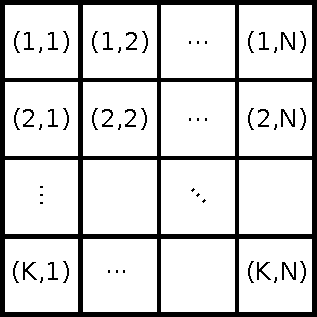
\includegraphics[width=\textwidth]{data_layouts.pdf}
      \caption{A simple 2-D data array with K rows and N columns.}
      \label{F:mem}
    \end{subfigure}
  \end{minipage}
  \hfil
  \begin{minipage}{0.45\linewidth}
    \begin{subfigure}[t]{\textwidth}
	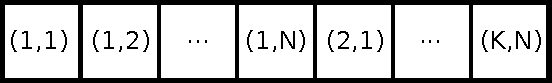
\includegraphics[width=\textwidth]{row_major.pdf}
	\caption{Row-major data ordering}
	\label{F:row_major}
    \end{subfigure}
    \\
    \begin{subfigure}[t]{\textwidth}
	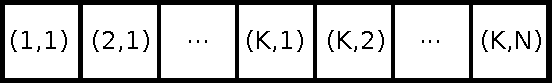
\includegraphics[width=\textwidth]{column_major.pdf}
	\caption{Column-major data ordering}
	\label{F:column_major}
    \end{subfigure}
  \end{minipage}
\end{figure}

When storing arrays for a chemical kinetic model, the data-storage layout and vectorization patterns are critical to achieving high-performance code.
\Cref{F:mem} depicts an example data array with K-rows and N-columns and index ($i$, $j$) corresponding to the $i$th row and $j$th column.
For example the concentration of species $j$ for the $i$-th thermo-chemical state would be stored in $[C]_{i, j}$ with $1 \le i \le N_{state}$, the number of thermo-chemical states considered, and $1 \le j \le \ns$, the number of species in the model.
The stored concentrations would then have $K = N_{\text{state}}$ rows, and $N = N_{\text{sp}}$ columns.

In the ``C'' (C row-major) format, the concentrations of all species for a single thermo-chemical condition $i$ would be stored sequentially in memory, i.e., with  $[C]_{1, 1}$ in index \num{1}, $[C]_{1, 2}$ in index \num{2} etc. as shown in \cref{F:row_major}.
Conversely in the ``F'' (Fortran column-major) format, the concentrations of a single species $j$ over all thermo-chemical states are adjacent in memory, corresponding to storing $[C]_{1, 1}$ in index \num{1}, $[C]_{2, 1}$ in index \num{2} and so on, as shown in \cref{F:column_major}.
This ordering---along with the device (CPU, GPU, etc.) and vectorization pattern in question---have a large effect on the performance of SIMD\slash SIMT-vectorized algorithms.

In a \textit{shallow}-SIMD\slash SIMT vectorization (also referred to as ``per-thread'' in previous works~\cite{Stone:2013aa} using GPUs), each SIMD-lane (or SIMT-thread) in a compute-unit evaluates thermo-chemical source terms\slash chemical kinetic Jacobian for a different thermo-chemical state.
If the data is stored in ``F''-order, the SIMD-lanes\slash SIMT-thread accessing $[C]_{1, j}\ldots[C]_{L, j}$, the concentration of species $j$ for states $1, 2,\ldots L$---the size of the vector lane for SIMD or the number of threads in a SIMT warp---will load sequential locations in memory.
The first $(j+1)$th species concentration however, $[C]_{1, j+1}$, will be $N_{\text{state}}$ memory locations away; this increases the likelihood of cache-misses on the CPU~\cite{gray2000rules}, but conversely is well suited to coalesced memory accesses on the GPU~\cite{NVIDIA:2018}.

In a \textit{deep}-SIMD\slash SIMT vectorization (also referred to as ``per-block'' in previous GPU works), a compute-unit utilizes its SIMD-lanes\slash SIMT-threads cooperatively to evaluate the thermo-chemical source terms for a single thermo-chemical state, thus SIMD-lanes loading $[C]_{1, j} \ldots [C]_{1, j + L}$---the species concentrations for state 1, species $j \ldots j + L$---will access sequential memory locations if the data is stored in ``C''-order.
Further, in the ``C''-ordering the furthest difference between any two species concentrations within the same thermo-chemical state is at most $N_{\text{sp}}$, with $N_{\text{sp}} \ll N_{\text{state}}$ in most cases; this greatly improved data-locality increases the chances of a cache-hit on the CPU, but leads to uncoalesced memory-accesses on the GPU.
However, a deep vectorization requires both synchronization between SIMD-lanes\slash SIMT-threads, and may result in SIMD-waste\slash SIMT thread-divergence, caused by different SIMD-lanes\slash SIMT-threads executing different instructions (e.g. resulting from different if\slash then branches)

\begin{figure}[htb]
  \centering
  \begin{minipage}{0.6\linewidth}
    \begin{subfigure}[t]{\textwidth}
	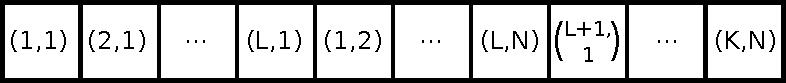
\includegraphics[width=\textwidth]{row_major_split.pdf}
	\caption{Row-major, wide-vectorized data ordering}
	\label{F:row_major_split}
    \end{subfigure}
    \\
    \begin{subfigure}[t]{\textwidth}
	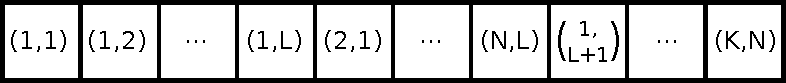
\includegraphics[width=\textwidth]{column_major_split.pdf}
	\caption{Column-major, deep-vectorized data ordering}
	\label{F:column_major_split}
    \end{subfigure}
  \end{minipage}
  \caption{Vectorized data ordering patterns}
  \label{F:vector_data}
\end{figure}

Finally,~\cref{F:vector_data} shows a vectorized data-ordering that improves the caching patterns of a shallow, ``C''-ordered SIMD vectorization on the CPU (\cref{F:row_major_split}) and a deep, ``F''-ordered SIMT vectorization on the GPU (\cref{F:column_major_split}).
This is accomplished by splitting the slower-varying axis of the data array---rows for ``C''-ordering, and columns for ``F''-ordering---into chunks of size $L$ (the SIMD vector-width, or SIMT warp-size) and laying these data out contigously in memory.
For example, using the data-ordering in~\cref{F:row_major_split}, the concentration of species $j$ for states $i\ldots i+L$, $[C]_{i, j} \ldots [C]_{i + L, j}$, are contiguous in memory and are followed by the concentration of species $j + 1$ for the same states, $[C]_{i, j + 1} \ldots [C]_{i + L, j + 1}$.
This pattern, similar to OpenCL's native vector data-types---e.g., \texttt{double\num{8}} which treats \num{8} contiguous double precision floating point numbers as a single vector datum---ensures that any SIMD operation occurs on data that is contiguous in memory, greatly improving caching and SIMD-throughput.
Conversely, the data-ordering in~\cref{F:column_major_split} is designed to enable coalesced memory accesses for ``F''-ordered, deep-SIMT vectorization on the GPU.
The effects of these various data-ordering and vectorization patterns on performance will be studied in~\cref{S:results}.

\subsection{Thermo-chemical Source Terms and Jacobian}
This new version of \texttt{pyJac} is capable of evaluating the thermo-chemical source terms for using both the constant-pressure (\conp) or constant-volume (\conv) assumption\footnote{Note: in this context, the ``constant-pressure'' and ``constant-volume'' assumptions refer to evaluation within a reaction sub-step in the operator splitting scheme, rather than a general constant-pressure or constant-volume reactive-flow simulation.}
In this section, we will only outline a brief summary of the system evaluated by \texttt{pyJac}; the interested reader is referred to our complete derivations, attached as supplemental material to this document.

The thermo-chemical state vector derivation consists of the temperature, the non-constant thermodynamic state parameter (volume or pressure) and the number of moles of all species except the last in the chemical model which is typically taken to be the bath-gas (e.g., \ce{N2}):
\loadeq{state}
where $T$ is the temperature, $V$ and $P$ the volume and pressure respectively, and $n_j$ the number of moles of the $j$th species in the model (containing $\ns$ total species).

This state vector---inspired by~\cite{SCHWER2002270}---has a number of features that recommend its use.
First, the state vector results in highly sparse chemical kinetic Jacobians as will be detailed in~\cref{S:sparsity}.
Second, mass is explicitly conserved in this formulation owing to the fact that the moles of the final species is calculated from the ideal gas law, and the rate of change of the final species from conservation of mass (see \cref{deriv-s:state,deriv-s:source} of the supplemental material respectively); i.e., system is not over-constrained.
Finally, the chemical kinetic Jacobian changes relatively little between the \conp~and \conv~forms, making maintaining the code-base much simpler.
Although most current combustion codes do not use species moles as a state variable, to\slash from more common mass\slash mole-fractions and moles is straightforward, and once inside integration of an chemical kinetic initial value problem, the choice of variables no longer matter.

The evolution of the thermo-chemical state vector is described by a set of chemical kinetic ordinary differential equations:
\loadeq{dstate}

For both \conp~and \conv, the molar source terms are~\cite{TurnsStephenR2012Aitc}:
\loadeq{dmolar}
where $\dot{\omega}_k$ is the $kth$ species' overall production rate:
\begin{equation}
 \dot{\omega}_{k} = \sum_{i=1}^{\nr} \nu_{k, i} R_{i} c_{i}
\end{equation}
where $\nu_{k, i}$ is the net stoichiometic coefficient of species $k$ in reaction $i$, $R_{i}$ the net rate of progress of reaction $i$ (described in~\cref{deriv-s:rop_net} of the supplemental), and $c_{i}$ the pressure modification term i.e., for third-body (see~\cref{deriv-s:thdbody} of the supplimental), or fall-off\slash chemically-activated reactions (\cref{deriv-s:falloff} of the same).

The temperature source term~\cite{TurnsStephenR2012Aitc} is:
\loadeq{dtemp}
where $H_k$, $U_k$, $C_{p,k}$ and $C_{v, k}$ are the enthalpy, internal energy, constant-pressure and constant-volume specific heat of species $k$ in molar units respectively, while $[C]_{k}$ is the concentration, given by:
\begin{equation}
 [C]_{k} = \frac{n_{k}}{V}
\end{equation}
By differentiating the ideal gas law, the volume and pressure source terms can be found:
\loadeq{dparam}
where $\mathcal{R}$ is the ideal gas-constant.

The Jacobian entries computed by \texttt{pyJac} are arranged such that entry ($i$, $j$) corresponds to the partial derivative of the $i$-th source term in~\cref{e:source_terms} by the $j$-th state variable in~\cref{e:state}:
\loadeq{jacgeneral}

The derivative of the temperature source term with respect to itself is:
\loadeq{dTdotdT}
and with respect to the thermodynamic state parameter (the volume \slash pressure for \conp\slash\conv~respectively):
\loadeq{dTdotdE}
and the moles of species $j$:
\loadeq{dTdotdnj}

The derivative of the thermodynamic state parameter with respect to the temperature is:
\loadeq{dEdotdT}
and with respect to itself:
\loadeq{dEdotdE}
and finally, by the moles of species $j$:
\loadeq{dEdotdnj}

The molar source terms are more complicated due to the derivatives of the net rate of progress---see~\cref{deriv-s:dropi}---and pressure modification terms---\cref{deriv-s:dci}---for the reactions.
The reader is again encouraged to read the supplimental material covering the exact derivations and forms of the reactions solved by \texttt{pyJac}.
The derivative of the molar source term with respect to temperature is:
\loadeq{dnkdotdT}
while, similarly the derivative with respect to the state parameter is:
\loadeq{dnkdotdE}
and the moles of species $j$:
\loadeq{dnkdotdnj}

\subsection{Code Generation and Testing Infrastructure}
Code generation is enabled by the python package \texttt{loo.py}~\cite{kloeckner_loopy_2014}, which translates user specified psuedo-code and data to OpenCL\slash C-code.
This allows for easy changes of program structure, e.g. data ordering, vectorization, threading patterns and easy switching of target-languages (and simpler extension to additional languages, e.g., CUDA).
Additionally, \texttt{loo.py} can execute developed subroutines from python (natively for C-code, and via \texttt{PyOpenCL}~\cite{kloeckner_pycuda_2012} for OpenCL-code), enabling unit-testing\slash validation for each component of the Jacobian or source terms.
The source-terms and subcomponents thereof (e.g., rates of progress, pressure-modification terms, etc.) are directly compared to Cantera~\cite{Cantera}, while the automatic differentiation code Adept~\cite{adept-v11} is used to obtain reference answers for Jacobian subcomponents.
The Portable OpenCL (POCL) implementation~\cite{poclIJPP} and OpenMP~\cite{dagum1998openmp} are used to run OpenCL and C unit-testing, respectively, on the continous integration framework Travis CI~\cite{travis:2018}.
Validation of the complete (as opposed to the subcomponent testing discussed here) generated source-terms and Jacobian codes will be discussed in detail in~\cref{s:validation}.


\section{Results and Discussion}
\subsection{Testing platforms and practical notes on OpenCL usage}

The performance and validation studies for this work were run on a variety of CPU and GPU platforms.
\Cref{t:cpus} shows the number of cores, vector instruction set and model of the CPUs used in this work; each CPU had both \texttt{v16.1.1} of the Intel OpenCL runtime~\cite{intelopencl:2018} and \texttt{v1.0} of the POCL~\cite{poclIJPP} runtime installed, each enabling OpenCL \texttt{v1.2} execution.
Additionally, \texttt{v5.0} of the LLVM\slash\texttt{clang}~\cite{Lattner:2004:LCF:977395.977673} compiler chain was installed on all machines to enable use of POCL.
In addition,~\cref{t:gpus} lists the model, number of CUDA cores and NVIDIA driver of each of the GPUs used in this work.
NVIDIA's OpenCL runtime is bundled with the NVIDIA driver~\cite{NVIDIA:2018}, hence we use driver version to specify the OpenCL runtime version.

Finally,~\cref{t:platforms} lists the platforms and vectorization\slash execution patterns they are capable of running.
It is important to note, that while OpenCL provides an easy way to enable cross-platform execution, there are some serious potential pit-falls in its use.
Typically speaking, the closed source OpenCL runtimes tested in this work (Intel and NVIDIA) contain more bugs that result in compilation failures or simply incorrect vectorized machine code; further, these runtimes (in our experience) tend to be less responsive to fixing said bugs, with relatively infrequent new releases (or in NVIDIAs case, change-logs of bugfixes).
As demonstration, we've created a minimum working example~\cite{nvidia_mwe} that demonstrates a failure of NVIDIA's OpenCL runtime corresponding to the GPU driver version \num{375.26} on a Tesla K40m GPU; by simply changing to another runtime (e.g., Intel), with no other code changes, the correct result can be found.
This provides a particularly vexing problem for the programmer, as there is often little that can be done to resolve the issue; thankfully, in this case we were able to upgrade the driver version to resolve the problem.

Further, the Intel and NVIDIA OpenCL runtimes lack a key feature---implementations of atomic operations on double precision variables---that are currently necessary for \texttt{pyJac} to run deep-vectorized code.
On the other hand, POCL is an open source OpenCL runtime that works on all CPU types tested in this work, and does implement these atomic operations; it is our experience that the POCL community is very responsive to bug reports and user outreach.
However, POCL's implicit vectorization module---which utilizes the LLVM compiler~\cite{Lattner:2004:LCF:977395.977673} to attempt to translate OpenCL code to vectorized machine code---typically fails to achieve much speedup, if any.
Thus POCL is a particularly useful tool for validation, but not necessarily for performance studies.
Thankfully, \texttt{loo.py} allows relatively easy switching between output languages; the only significant code change is building the wrapper that initializes\slash transfers memory and calls the kernel.
Indeed, the OpenMP code-generation built into \texttt{pyJac} is currently only capable of parallel-execution, but extending this platform to shallow\slash deep-vectorizations (via \texttt{loo.py}) is a key priority going forwards.
This discussion will be expanded upon in~\cref{s:future} to highlight the most promising future directions.


\begin{table}[htb]
\centering
\begin{tabular}{@{}l l l@{}}
\toprule
CPU Model        & Xeon X5650      & E5-2690 V3     \\
\midrule
Instruction Set  & SSE4.2 	   & AVX2 	    \\
Vector Width     & \SI{128}{\bit}  & \SI{256}{\bit} \\
Cores            & $2 \times 6$    & $2 \times 12$  \\
Identifier       & \texttt{sse4.2} & \texttt{avx2}  \\
OpenCL Version   & \num{1.2}       & \num{1.2}      \\
\bottomrule
\end{tabular}
\caption{The Intel CPU configurations used in this study. The identifier field will be used as a shorthand descriptor in the performance plots to quickly identify the CPU type.}
\label{t:cpus}
\end{table}

\begin{table}
\centering
\begin{tabular}{@{}l l l l l@{}}
\toprule
NVIDIA Model   & Tesla C2075    & Tesla K40m    \\
\midrule
Driver Version & \num{384.81}   & \num{387.26}  \\
CUDA Cores     & \num{448}      & \num{2880}    \\
Identifier     & \texttt{C2075} & \texttt{K40m} \\
OpenCL Version & \num{1.1}	& \num{1.2}	\\
\bottomrule
\end{tabular}
\caption{The NVIDIA GPU configurations used in this study.  NVIDIA's OpenCL runtime is provided with the graphic driver, rather than any specific version of CUDA.
Again, the identifier field will be used as a shorthand descriptor during analysis of the performance results.}
\label{t:gpus}
\end{table}

\begin{table}
\centering
\begin{tabular}{@{}l c c c@{}}
\toprule
Platform & Parallel & Shallow Vectorization & Deep Vectorization \\
\midrule
OpenMP & X & -- & -- \\
POCL OpenCL & X & X & X \\
Intel OpenCL & X & X & -- \\
NVIDIA OpenCL & -- & X & -- \\
\bottomrule
\end{tabular}
\caption{The various platforms used in this study and the execution \slash vectorization patterns they are capable of running}
\label{t:platforms}
\end{table}


\subsection{Source term validation}
\label{s:validation}
The reaction rates of progress (ROP), species and temperature rates in this study are validated by comparison with Cantera~\cite{Cantera}, however special care must be taken due floating point arithmetic issues.

For a direct comparison, a relative error norm of a quantity $X_{ij}$ over all states $j$, and reactions (or species) $i$ was computed using the $L^{\infty}$ norm:
\begin{equation}
E_{X} = \left\lVert \frac{\left\lvert X_{ij,\text{CT}} - X_{ij}\right\rvert}{\num{e-10} + \num{e-6} * \left\lvert X_{ij,\text{CT}} \right\rvert} \right\rVert_{i,j,\infty}
\label{e:rel_err}
\end{equation}
where the \text{CT} subscript indicates values from Cantera~\cite{Cantera}

However, in computing the net ROP of reaction $i$ for state $j$ from the forward and reverse ROP: $R_{ij} = R_{ij}^{\prime} - R_{ij}^{\prime\prime}$, accuracy can easily be lost as the net ROP may be---particularly near chemical equilibrium---many orders of magnitude smaller than the forward or reverse rates.
To quantify this phenomena, the error in forward ROP is first defined as:
\begin{equation}
\varepsilon^{\prime}_{ij} = \left\lvert R_{ij}^{\prime} - R_{ij,\text{CT}}^{\prime} \right\rvert
\end{equation}
while the error in reverse ROP, $\varepsilon^{\prime\prime}_{ij}$, can be defined analogously.
Finally, for the reaction $i^{*}$ and state $j^{*}$ that result in the largest error in net ROP, i.e. $E_{R}$, an estimate of the error attributable to floating point error accumulation from the forward and reverse ROPs can be obtained as:
\begin{equation}
E_{\varepsilon} = \frac{\max(\varepsilon^{\prime}_{i^{*}j^{*}}\text{, }\varepsilon^{\prime\prime}_{i^{*}j^{*}})}{\num{e-10} + \num{e-6} * \left\lvert R_{i^{*}j^{*},\text{CT}} \right\rvert}
\end{equation}
This estimate allows for direct comparison of the error in forward or reverse ROPs to the value of the net ROP itself, if they are of similar magnitude the error in net ROP will be large.

\begin{table}[htb]
\sisetup{retain-zero-exponent=true}
\centering
\begin{tabular}{@{}l S[table-format=1.2e1] S[table-format=1.2e1] S[table-format=1.2e1] S[table-format=1.2e1]@{}}
\toprule
\multicolumn{1}{l}{Model} & \multicolumn{1}{l}{\ce{H2}\slash~\ce{CO}\cite{Burke:2011fh}} & \multicolumn{1}{l}{GRI-Mech.~3.0\cite{smith_gri-mech_30}} & \multicolumn{1}{l}{USC-Mech II\cite{Wang:2007}} & \multicolumn{1}{l}{\ce{iC5H11OH}\cite{Sarathy:2013jr}} \\
\midrule
\multicolumn{1}{c}{$E_{R^{\prime}}$}                    & 1.56e-8 & 2.95e-8 & 9.42e-8 & 4.86e-4 \\
\multicolumn{1}{c}{$E_{R^{\prime\prime}}$}              & 6.92e-8 & 6.53e-8 & 1.20e-7 & 5.07e-4 \\
\multicolumn{1}{c}{$E_{R}$}                             & 1.49e1  & 1.11e0  & 2.80e0  & 4.82e-1 \\
\multicolumn{1}{c}{$E_{\varepsilon}$}                   & 1.48e1  & 1.13e0  & 2.93e0  & 5.03e-1 \\
\multicolumn{1}{c}{$E_{\frac{\text{d} n}{\text{d} t}}$} & 2.53e1  & 2.60e0  & 7.62e0  & 1.58e1 \\
\multicolumn{1}{c}{$E_{\frac{\text{d} T}{\text{d} t}}$} & 3.94e5  & 3.35e8  & 3.95e6  & 7.11e7 \\
\multicolumn{1}{c}{$E_{\frac{\text{d} S}{\text{d} t}}$} & 3.52e12 & 3.46e12 & 3.44e12 & 3.38e12 \\
\bottomrule
\end{tabular}
\caption{Summary of rate of progress, species and temperature rate correctness.
Error statistics are based on the infinity-norm of the relative error detailed in Eq.~\eqref{e:rel_err} for each quantity.
The ``S'' in $E_{\frac{\text{d} S}{\text{d} t}}$ refers to the thermodynamic state parameter, either $V$ or $P$ for \conp~and \conv~respectively.
}
\label{T:source_error}
\end{table}

In Table~\ref{T:source_error}, we see the results of this code as compared to Cantera~\cite{Cantera} on a library of partially stirred reaction conditions (PaSR) described in our previous works~\cite{CurtisGPU:2017,Niemeyer:2016aa}.
Very close agreement is observed for the forward and reverse ROP for all models, however the error norm is \textasciitilde\numrange{3}{4} orders of magnitude larger for the isopentanol model.
This results from differences in evaluation of P-Log reactions between \texttt{pyJac} and Cantera; namely \texttt{pyJac} computes the logarithm of the upper and lower reaction Arrhenius rates (see~\cref{deriv-s:pdep}) analytically while Cantera evaluates this term numerically.
If the error from P-Log reactions are not considered in~\cref{e:rel_err}, the forward and reverse ROP falls to \num{5.44e-08} and \num{1.59e-07} respectively.
We note that this discrepancy does not imply any incorrectness in either \texttt{pyJac} or Cantera---in fact, the error is still well within the proscribed tolerances in~\cref{e:rel_err}---but merely emphasizes the effect small code-changes can have on the accumulation of floating point errors.

This point is further underscored by the error in the net ROP, which is \textasciitilde\numrange{3}{9} orders of magnitude (or \numrange{7}{9} orders of magnitude for the P-Log excluded error) larger than the error in either the forward or reverse ROP.
In~\cref{T:source_error}, we see that $E_{\varepsilon}$ is very similar in magnitude to $E_R$ in all cases, indicating that this large increase in error is caused by the accumulation of floating point error from the forward and reverse ROPs, as previously discussed.
The molar species production rate error norm is similar in magnitude to that of the net ROP, however the temperature and state parameter rate errors again increases as the error in net species production rates is amplified by multiplication with thermodynamic properties.
Again, we note that the above discussion does not imply that discrepencies in computation of the net ROP will cause large error in chemical kinetic integration---either in this code or Cantera~\cite{Cantera}---as this loss of accuracy only occurs when the forward and reverse ROP are nearly equal, implying the reaction is in near-equilibrium.

\subsection{Jacobian validation}

As in our previous work~\cite{Niemeyer:2016aa}, the correctness of the Jacobian codes generated by \texttt{pyJac} was determined by comparison to the Jacobian obtained by automatic differentiation of the source rate subroutines generated by \texttt{pyJac} via the \texttt{Adept} software library~\cite{adept-v11,hogan2014fast}.
The reasons for this choice are explained fully in~\cite{Niemeyer:2016aa}, but broadly speaking automatic differentiation provides relatively fast, highly accurate Jacobian matrix evaluation with minimal additional programming little effort.
The discrepancy between the analytical and automatic differentiated Jacobians for thermo-chemical state $k$, denoted by $\mathcal{J}_k$ and $\hat{\mathcal{J}}_k$ respectively, is determined by the relative error Frobenius norm over all Jacobian indicies $i, j$:
\begin{equation}
 \label{e:jac_error_base}
 E_{\text{rel}, k} = \frac{\left\lVert \hat{\mathcal{J}}_{ijk} - \mathcal{J}_{ijk} \right\rVert_{i,j,F}}{\left\lVert \hat{\mathcal{J}}_{ijk} \right\rVert_{i,j,F}}
\end{equation}

To avoid large relative errors of small nonzero Jacobian elements due to accumulation of floating point error, the Frobenius norm of the automatically differentiated Jacobian is calculated over all thermo-chemical states $k$:
\begin{equation}
 \label{e:thresh}
 \mathcal{T} = \left\lVert \mathcal{\hat{J}} \right\rVert_{k, F}
\end{equation}
The error statistics reported in this section are then based only on matrix elements where $\mathcal{J}_{ijk} \ge \frac{\mathcal{T}}{\mathcal{C}}$; this filtered form of~\cref{e:jac_error_base} is denoted $E_{\mathcal{C}}$.

\begin{table}[tbp]
\centering
\begin{tabular}{@{}l S S[table-format=1.3e1] S[table-format=1.3e1] S[table-format=1.3e1]@{}}
\toprule
Model                 & \multicolumn{1}{c}{Sample size}   & \multicolumn{1}{c}{$\bar{\mathcal{T}}$}  & \multicolumn{1}{c}{$E_{10^{20}}$}   & \multicolumn{1}{c}{$E_{10^{15}}$} \\
\midrule
\ce{H2}\slash \ce{CO} & \num{900900}                      & \num{6.431e+18}      & \num{8.084e-1}  & \num{1.907e-5} \\
GRI-Mech 3.0          & \num{450900}                      & \num{7.783e+19}      & \num{1.890e-7}  & \num{1.877e-7} \\
USC-Mech II           & \num{91800}                       & \num{2.830e+21}      & \num{1.540e-3}  & \num{1.704e-7} \\
\ce{iC5H11OH}         & \num{450900}                      & \num{2.733e+26}      & \num{1.363e-3}  & \num{2.764e-5} \\
\bottomrule
\end{tabular}
\caption{Summary of Jacobian matrix validation results.
Error statistics are the largest filtered relative error $E_\mathcal{C}$ for over all samples.
It is noted that the threshold described in~\cref{e:thresh} varies slightly between the \conp~and \conv~cases; the reported $\bar{\mathcal{T}}$ is the average of the two, however the appropriate value was used during calculations of the error statistics..
}
\label{T:error}
\end{table}

\Cref{T:error} presents the error statistics of \texttt{pyJac} over the tested PaSR thermo-chemical condition database.
For all tested cases, the maximum filtered error norm is less than unity.
The filtered error norm is largest for the \ce{H2}\slash\ce{CO} model with the more stringent tolerance ($\mathcal{C} = 10^{20}$).
We note that $\mathcal{T}$ for this model is smaller than the tolerance in this case, and hence we are comparing numbers smaller than $\mathcal{O}(1)$; relaxing the tolerance to $\mathcal{C} = 10^{15}$ significantly lowers the filtered error norm to $\mathcal{O}(10^{-5})$.
Similar error characteristics are seen for all models except GRI-Mech 3.0---in which the error norms for both tolerances are $\sim\mathcal{O}(10^{-7})$---that is a larger error norm for the more stringent tolerance that drops 2--4 orders of magnitude for the relaxed tolerance.

\subsection{Sparsity patterns}
\label{S:sparsity}

In general, the Jacobian matrices generated by \texttt{pyJac} are largely sparse with non-zero entries mainly corresponding to species that participate in the same reaction (or non-default efficiency third-body species in a reaction), and mostly dense rows \slash columns corresponding to the temperature and thermodynamic state parameter.
However, the explicit-mass conservation formulation of \texttt{pyJac} can introduce additional non-zero entries in two ways.
First, if the last-species in the model (i.e., the bath-gas) participates directly in a reaction, the derivative of the forward or reverse rate of progress with respect to any other species is non-zero (see~\cref{deriv-s:dri_dnj}).
Similarly, if the last-species has a third-body efficiency not equal to the default (unity), this will again force all the derivative of the pressure-modification term with respect to other species to be non-zero (see~\cref{deriv-s:dci_thd}).
Either case will result in an undesirable fully dense Jacobian row for all species that have a non-zero net stoichiometic coefficient in such a reaction.

However, \texttt{pyJac} allows the user to simply ignore these derivatives (via a command-line switch) to and avoid any negative adverse affects on the Jacobian sparsity.
The rational behind this choice is that many common implicit integration techniques (e.g., CVODE~\cite{cvode:2.8.2}) used in solution of chemical kinetic initial value problems are formulated around the assumption that the supplied Jacobian is approximate; this allows the Jacobian and its LU factorization to be reused for multiple internal integration time-steps, accelerating the solution process.
For such solvers, there is no need for the exact form of the Jacobian and the so-called ``approximate'' form is preferable.
Hence, in this section we will detail the sparsity of both forms of the Jacobian for the chemical models tested.

In~\cref{F:jac_sparsity}, a graphical representation of the sparsity pattern for GRI-Mech 3.0 is displayed.
In particular we note that~\cref{F:jac_sparse_approx} is has several rows that are no longer fully-dense, as result of its approximate form -- these rows correspond to species directly interacting with \ce{N2}, largely in GRI-Mech 3.0's \ce{NOx} chemistry reactions.
\cref{T:jac_sparsity} shows the density of the exact and approximate Jacobians for all mechanisms tested in this work.
The smallest model, \ce{H2}\slash\ce{CO} is very dense with \textasciitilde\SI{70}{\percent} of the Jacobian entries non-zero however this drops to just \textasciitilde\SI{50}{\percent} for GRI-Mech 3.0, and continues to decrease to \textasciitilde\SI{27}{\percent} for USC-Mech II and just \textasciitilde\SI{10}{\percent} for the isopentanol model.
The approximate Jacobian assumption drops the density of Jacobian by \textasciitilde\SIrange{3}{7}{\percent} for all models.

\begin{figure}[htb]
  \centering
  \begin{subfigure}{0.45\linewidth}
      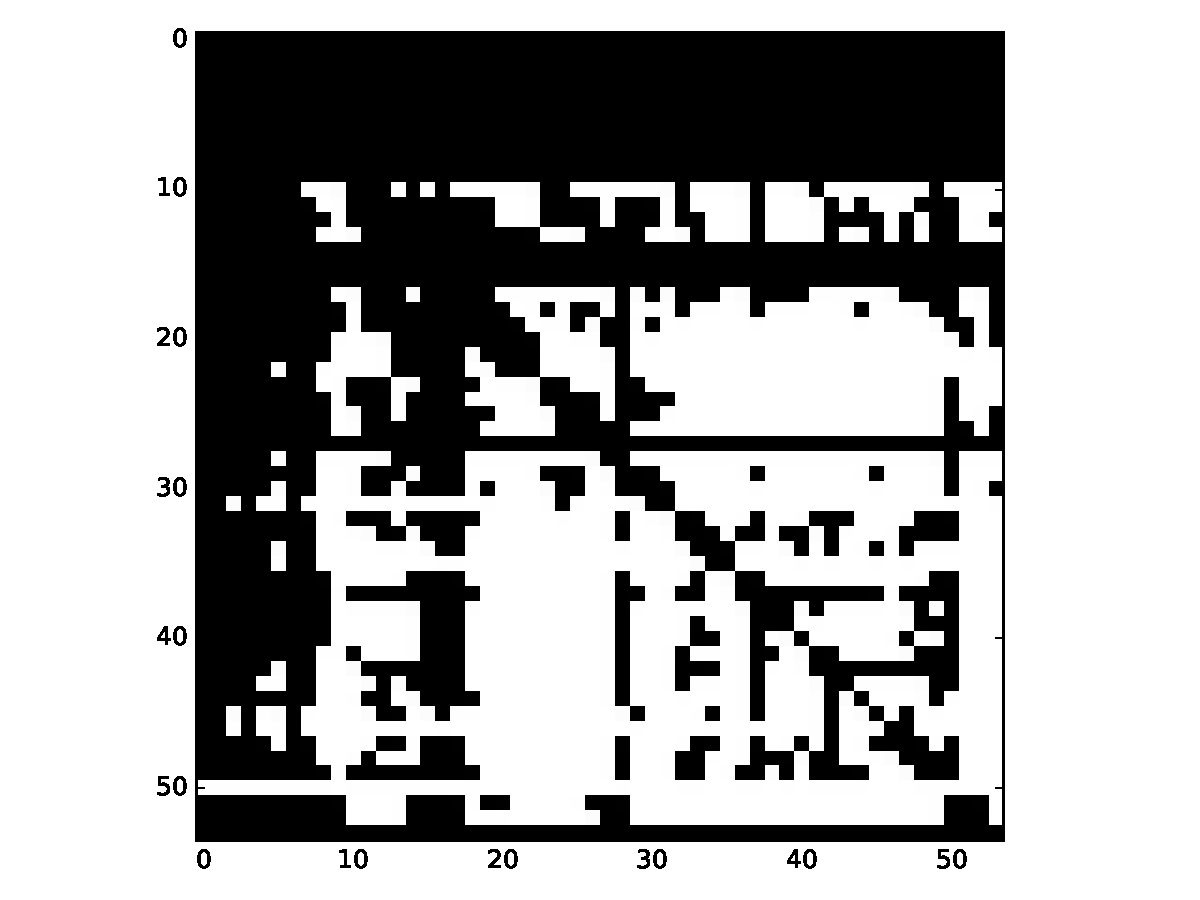
\includegraphics[width=\textwidth]{ch4_sparsity_exact.pdf}
      \caption{The ``exact'' Jacobian.}
      \label{F:jac_sparse_exact}
  \end{subfigure}
  \hfill
  \begin{subfigure}{0.45\linewidth}
      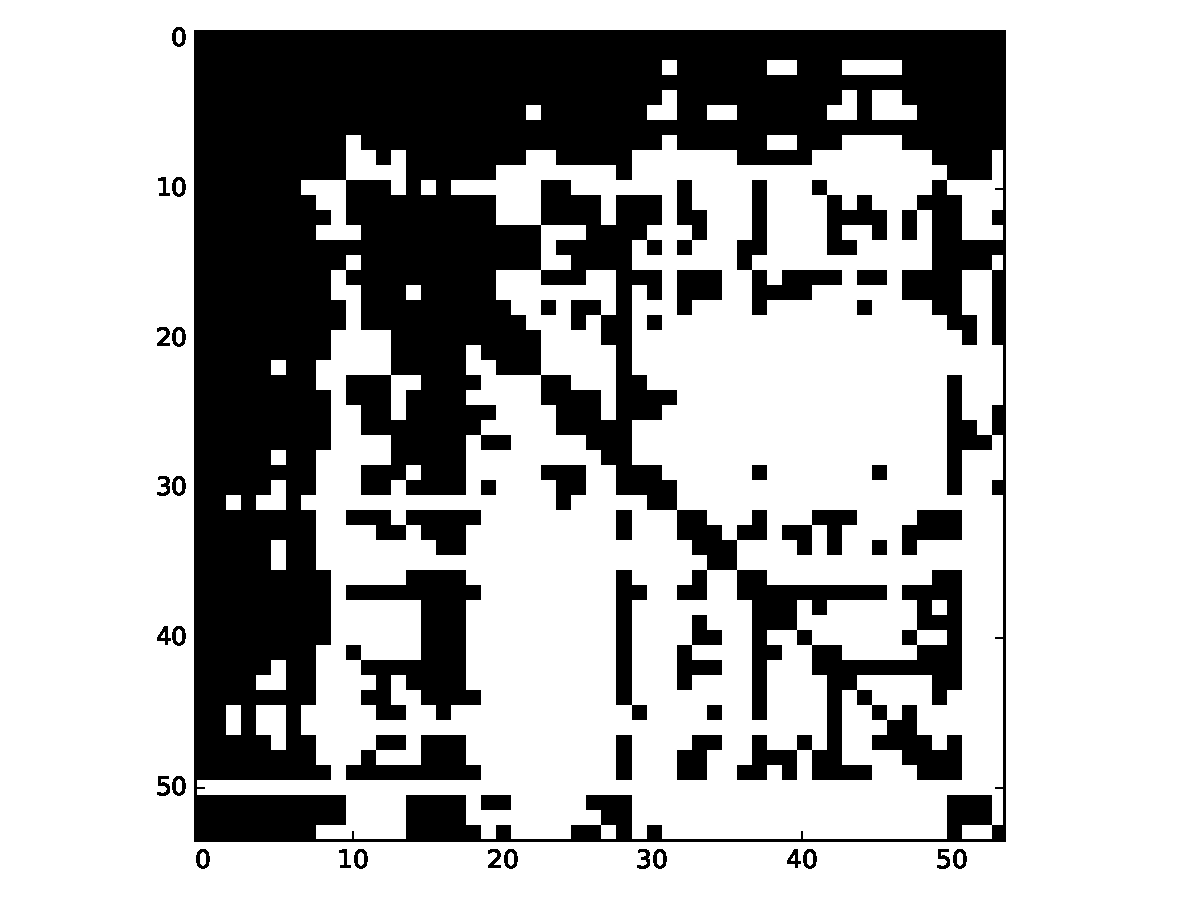
\includegraphics[width=\textwidth]{ch4_sparsity_approximate.pdf}
      \caption{The ``approximate'' Jacobian.}
      \label{F:jac_sparse_approx}
  \end{subfigure}
  \caption{A graphical representation of the sparsity pattern of the chemical kinetic Jacobian generated by \texttt{pyJac} for GRI-Mech 3.0.
	   Black squares indicate a non-zero Jacobian entry, while white square correspond to an empty entry.
	   The numbers indicate the index of the entry in the state vector.}
  \label{F:jac_sparsity}
\end{figure}

\begin{table}[tbp]
\centering
\begin{tabular}{@{}l S[table-format=2.1] S[table-format=2.1]@{}}
\toprule
Model                 & \multicolumn{1}{c}{Exact Jacobian Density} & \multicolumn{1}{c}{Approximate Jacobian Density} \\
\midrule
\ce{H2}\slash \ce{CO} & \SI{71.4}{\percent} & \SI{68.4}{\percent} \\
GRI-Mech 3.0          & \SI{56.7}{\percent} & \SI{49.8}{\percent} \\
USC-Mech II           & \SI{28.2}{\percent} & \SI{26.4}{\percent} \\
\ce{iC5H11OH}         & \SI{11.5}{\percent} & \SI{7.98}{\percent} \\
\bottomrule
\end{tabular}
\caption{The density of the exact and approximate Jacobians generated by \texttt{pyJac} for the various models studied.}
\label{T:jac_sparsity}
\end{table}



\subsection{Performance}
\label{S:results}
The performance studies in this work were run on the platforms listed in~\cref{t:cpus,t:gpus}.
Runtimes in each case were averaged over ten runs, each using the same set of PaSR conditions utilized in validation.
The wrapping code---responsible for initializing\slash transfering memory, reading input, etc.---was compiled with \texttt{gcc v5.4.0} on the \texttt{avx2}\slash\texttt{K40m} platforms, and \texttt{gcc 4.8.5} on the \texttt{sse4.2}\slash\texttt{C2075} machines.
The optimization level ``\texttt{-O3}'' was used in all cases, and no ``fast-math'' OpenCL optimizations were enabled.
Additionally, the ``exact'' form of the Jacobian (as opposed the the ``appropriate'' form discussed in~\cref{S:sparsity}) was used in all cases.

\Cref{f:source} shows the runtime of \texttt{pyJac} on the test platforms.

\begin{figure}[htb]
   \centering
  \begin{subfigure}{0.45\linewidth}
      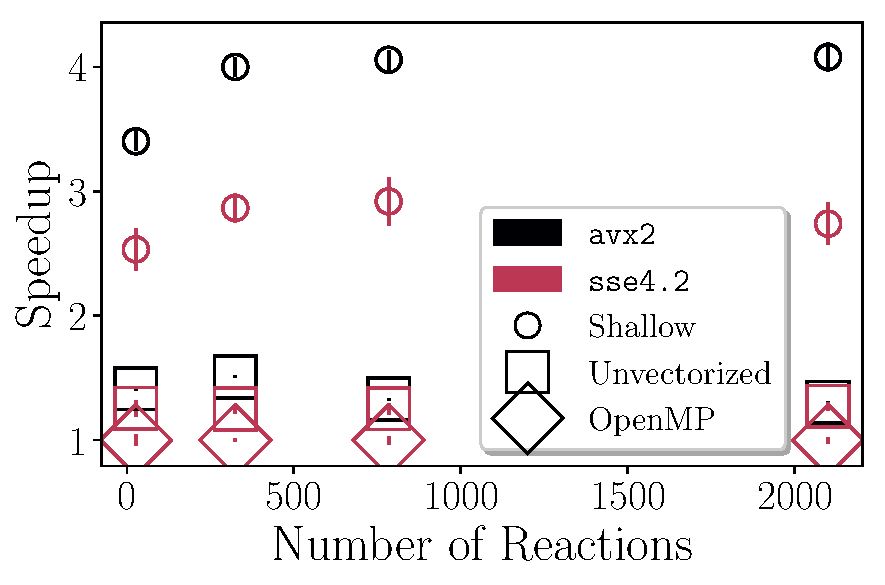
\includegraphics[width=\textwidth]{intel_source.pdf}
      \caption{The ``exact'' Jacobian.}
      \label{F:intel_source_noorm}
  \end{subfigure}
 \label{f:source}
\end{figure}


\section{Future directions}
\label{s:future}
NVIDIA 375.26 is a bad driver, yo.

\section{Conclusions}
In this work, automatically generated OpenCL codes for shallow SIMD-vectorized thermo-chemical source term evaluation were developed and validated against Cantera~\cite{Cantera} for a wide range of chemical kinetic models~\cite{Burke:2011fh,smith_gri-mech_30,Wang:2007,Sarathy:2013jr}.
Significant speedups of up to \SIrange{1.90}{2.45}{$\times$} over a baseline SIMT-vectorized code were observed.
Two data-ordering schemes were investigated, showing a clear performance benefit for use of the ``C'' (row-major) ordering for the shallow vectorized code.
Further, this study suggests that a deep SIMD-vectorized code---currently under development---may see even greater accelerations due to expected increases in cache-hit rates.
Larger vector-widths were found to provide accelerations for the smaller models studied, but the speedup was similar over all vector-widths tested for the largest models investigated.
Finally, the strong parallel scaling efficiency was examined for the shallow vectorized code; the larger models exhibited higher scaling efficiency, possibly due to failure of the \ce{H2}\slash\ce{CO} model to saturate the CPU throughput.
Future extensions of this work will include development of a SIMD\slash SIMT-accelerated sparse-analytical Jacobian code targeted at CPUs, GPUs, and MICs.

\section{Acknowledgements}
This research was funded by the National Science Foundation under grant ACI-1534688.

\bibliography{paper}

\end{document}
